% Options for packages loaded elsewhere
\PassOptionsToPackage{unicode}{hyperref}
\PassOptionsToPackage{hyphens}{url}
\documentclass[
]{book}
\usepackage{xcolor}
\usepackage{amsmath,amssymb}
\setcounter{secnumdepth}{5}
\usepackage{iftex}
\ifPDFTeX
  \usepackage[T1]{fontenc}
  \usepackage[utf8]{inputenc}
  \usepackage{textcomp} % provide euro and other symbols
\else % if luatex or xetex
  \usepackage{unicode-math} % this also loads fontspec
  \defaultfontfeatures{Scale=MatchLowercase}
  \defaultfontfeatures[\rmfamily]{Ligatures=TeX,Scale=1}
\fi
\usepackage{lmodern}
\ifPDFTeX\else
  % xetex/luatex font selection
\fi
% Use upquote if available, for straight quotes in verbatim environments
\IfFileExists{upquote.sty}{\usepackage{upquote}}{}
\IfFileExists{microtype.sty}{% use microtype if available
  \usepackage[]{microtype}
  \UseMicrotypeSet[protrusion]{basicmath} % disable protrusion for tt fonts
}{}
\makeatletter
\@ifundefined{KOMAClassName}{% if non-KOMA class
  \IfFileExists{parskip.sty}{%
    \usepackage{parskip}
  }{% else
    \setlength{\parindent}{0pt}
    \setlength{\parskip}{6pt plus 2pt minus 1pt}}
}{% if KOMA class
  \KOMAoptions{parskip=half}}
\makeatother
\usepackage{color}
\usepackage{fancyvrb}
\newcommand{\VerbBar}{|}
\newcommand{\VERB}{\Verb[commandchars=\\\{\}]}
\DefineVerbatimEnvironment{Highlighting}{Verbatim}{commandchars=\\\{\}}
% Add ',fontsize=\small' for more characters per line
\usepackage{framed}
\definecolor{shadecolor}{RGB}{248,248,248}
\newenvironment{Shaded}{\begin{snugshade}}{\end{snugshade}}
\newcommand{\AlertTok}[1]{\textcolor[rgb]{0.94,0.16,0.16}{#1}}
\newcommand{\AnnotationTok}[1]{\textcolor[rgb]{0.56,0.35,0.01}{\textbf{\textit{#1}}}}
\newcommand{\AttributeTok}[1]{\textcolor[rgb]{0.13,0.29,0.53}{#1}}
\newcommand{\BaseNTok}[1]{\textcolor[rgb]{0.00,0.00,0.81}{#1}}
\newcommand{\BuiltInTok}[1]{#1}
\newcommand{\CharTok}[1]{\textcolor[rgb]{0.31,0.60,0.02}{#1}}
\newcommand{\CommentTok}[1]{\textcolor[rgb]{0.56,0.35,0.01}{\textit{#1}}}
\newcommand{\CommentVarTok}[1]{\textcolor[rgb]{0.56,0.35,0.01}{\textbf{\textit{#1}}}}
\newcommand{\ConstantTok}[1]{\textcolor[rgb]{0.56,0.35,0.01}{#1}}
\newcommand{\ControlFlowTok}[1]{\textcolor[rgb]{0.13,0.29,0.53}{\textbf{#1}}}
\newcommand{\DataTypeTok}[1]{\textcolor[rgb]{0.13,0.29,0.53}{#1}}
\newcommand{\DecValTok}[1]{\textcolor[rgb]{0.00,0.00,0.81}{#1}}
\newcommand{\DocumentationTok}[1]{\textcolor[rgb]{0.56,0.35,0.01}{\textbf{\textit{#1}}}}
\newcommand{\ErrorTok}[1]{\textcolor[rgb]{0.64,0.00,0.00}{\textbf{#1}}}
\newcommand{\ExtensionTok}[1]{#1}
\newcommand{\FloatTok}[1]{\textcolor[rgb]{0.00,0.00,0.81}{#1}}
\newcommand{\FunctionTok}[1]{\textcolor[rgb]{0.13,0.29,0.53}{\textbf{#1}}}
\newcommand{\ImportTok}[1]{#1}
\newcommand{\InformationTok}[1]{\textcolor[rgb]{0.56,0.35,0.01}{\textbf{\textit{#1}}}}
\newcommand{\KeywordTok}[1]{\textcolor[rgb]{0.13,0.29,0.53}{\textbf{#1}}}
\newcommand{\NormalTok}[1]{#1}
\newcommand{\OperatorTok}[1]{\textcolor[rgb]{0.81,0.36,0.00}{\textbf{#1}}}
\newcommand{\OtherTok}[1]{\textcolor[rgb]{0.56,0.35,0.01}{#1}}
\newcommand{\PreprocessorTok}[1]{\textcolor[rgb]{0.56,0.35,0.01}{\textit{#1}}}
\newcommand{\RegionMarkerTok}[1]{#1}
\newcommand{\SpecialCharTok}[1]{\textcolor[rgb]{0.81,0.36,0.00}{\textbf{#1}}}
\newcommand{\SpecialStringTok}[1]{\textcolor[rgb]{0.31,0.60,0.02}{#1}}
\newcommand{\StringTok}[1]{\textcolor[rgb]{0.31,0.60,0.02}{#1}}
\newcommand{\VariableTok}[1]{\textcolor[rgb]{0.00,0.00,0.00}{#1}}
\newcommand{\VerbatimStringTok}[1]{\textcolor[rgb]{0.31,0.60,0.02}{#1}}
\newcommand{\WarningTok}[1]{\textcolor[rgb]{0.56,0.35,0.01}{\textbf{\textit{#1}}}}
\usepackage{longtable,booktabs,array}
\usepackage{calc} % for calculating minipage widths
% Correct order of tables after \paragraph or \subparagraph
\usepackage{etoolbox}
\makeatletter
\patchcmd\longtable{\par}{\if@noskipsec\mbox{}\fi\par}{}{}
\makeatother
% Allow footnotes in longtable head/foot
\IfFileExists{footnotehyper.sty}{\usepackage{footnotehyper}}{\usepackage{footnote}}
\makesavenoteenv{longtable}
\usepackage{graphicx}
\makeatletter
\newsavebox\pandoc@box
\newcommand*\pandocbounded[1]{% scales image to fit in text height/width
  \sbox\pandoc@box{#1}%
  \Gscale@div\@tempa{\textheight}{\dimexpr\ht\pandoc@box+\dp\pandoc@box\relax}%
  \Gscale@div\@tempb{\linewidth}{\wd\pandoc@box}%
  \ifdim\@tempb\p@<\@tempa\p@\let\@tempa\@tempb\fi% select the smaller of both
  \ifdim\@tempa\p@<\p@\scalebox{\@tempa}{\usebox\pandoc@box}%
  \else\usebox{\pandoc@box}%
  \fi%
}
% Set default figure placement to htbp
\def\fps@figure{htbp}
\makeatother
\setlength{\emergencystretch}{3em} % prevent overfull lines
\providecommand{\tightlist}{%
  \setlength{\itemsep}{0pt}\setlength{\parskip}{0pt}}
\usepackage[]{natbib}
\bibliographystyle{plainnat}
\usepackage{booktabs}
\usepackage{bookmark}
\IfFileExists{xurl.sty}{\usepackage{xurl}}{} % add URL line breaks if available
\urlstyle{same}
\hypersetup{
  pdftitle={Bivariate Linear Regression},
  pdfauthor={Samuel Rowe adapted from Acock (2023)},
  hidelinks,
  pdfcreator={LaTeX via pandoc}}

\title{Bivariate Linear Regression}
\author{Samuel Rowe adapted from Acock (2023)}
\date{2026-11-17}

\begin{document}
\maketitle

{
\setcounter{tocdepth}{1}
\tableofcontents
}
\begin{Shaded}
\begin{Highlighting}[]
\NormalTok{bookdown}\SpecialCharTok{::}\FunctionTok{render\_book}\NormalTok{()}
\end{Highlighting}
\end{Shaded}

\chapter*{Overview}\label{overview}
\addcontentsline{toc}{chapter}{Overview}

Topics:

\begin{enumerate}
\def\labelenumi{\arabic{enumi}.}
\tightlist
\item
  Bivariate Linear Regression
\item
  Exercises
\end{enumerate}

\chapter{Simple Linear Regression in Stata}\label{simple-linear-regression-in-stata}

Our model for a simple bivariate linear regression is the following:

\[ y_i = \beta_0 + \beta_1 x_i + \varepsilon_i\]

\section{Simple Linear Regression Model}\label{simple-linear-regression-model}

Using the 2006 General Social Survey, we will look at the association between occupational prestige and hours worked. We will set up our bivariate linear regression model as the following:

\[ prestige80_i=\beta_0 + \beta_1 hrs_i + \varepsilon_i \]

\subsection{Set up your null hypothesis}\label{set-up-your-null-hypothesis}

Next, we will set up a null hypothesis:

\[ H_{0}: \beta_1 = 0 \]

\[ H_{a}: \beta_1 \neq 0 \]

Notice for that this will use a two-tailed test instead of a one tailed test. We can set \(\alpha=0.05\), so we will need to look up the critical \(t\) value for \(t_{0.05/2}\) or \(t_{0.025}\).

\subsection{Descriptive Statistics}\label{descriptive-statistics}

First, let's look at the descriptive statistics

\begin{Shaded}
\begin{Highlighting}[]
\NormalTok{cd }\StringTok{"/Users/Sam/Desktop/Econ 643/AGIS/"}
\KeywordTok{use}\NormalTok{ gss2006\_chapter8\_selected, }\KeywordTok{clear}
\KeywordTok{summarize}\NormalTok{ prestg80 hrs1}
\end{Highlighting}
\end{Shaded}

\begin{verbatim}
/Users/Sam/Desktop/Econ 643/AGIS

(General Social Surveys, 1972-2006 [Cumulative File], Dataset 0001)

    Variable |        Obs        Mean    Std. dev.       Min        Max
-------------+---------------------------------------------------------
    prestg80 |      4,270    44.16745    13.99946         17         86
        hrs1 |      2,739    42.07631    14.23166          1         89
\end{verbatim}

We can see that the dependent variable's mean is 44.2 with a standard deviation of 14.0 and its range is \([17, 86]\). The independent variable's mean is 42.1 hours with a standard deviation of 14.2 hours and its range is \([1,89]\) hours per week.

\textbf{Note:} There are 4,270 observations with occupational prestige, but only 2,739 have reported hours per week.

\subsection{Simple Bivariate Linear Regression}\label{simple-bivariate-linear-regression}

Next, we will use the \textbf{regress} command to run a linear regression. We use \textbf{regress \(y\) \(x\)} to regress \(y\) onto \(x\).

\begin{Shaded}
\begin{Highlighting}[]
\KeywordTok{regress}\NormalTok{ prestg80 hrs1}
\end{Highlighting}
\end{Shaded}

\begin{verbatim}
      Source |       SS           df       MS      Number of obs   =     2,715
-------------+----------------------------------   F(1, 2713)      =     67.32
       Model |   13125.035         1   13125.035   Prob > F        =    0.0000
    Residual |  528901.224     2,713  194.950691   R-squared       =    0.0242
-------------+----------------------------------   Adj R-squared   =    0.0239
       Total |  542026.259     2,714  199.714908   Root MSE        =    13.962

------------------------------------------------------------------------------
    prestg80 | Coefficient  Std. err.      t    P>|t|     [95% conf. interval]
-------------+----------------------------------------------------------------
        hrs1 |   .1546416   .0188468     8.21   0.000      .117686    .1915972
       _cons |   38.14733   .8362129    45.62   0.000     36.50765    39.78701
------------------------------------------------------------------------------
\end{verbatim}

Let's look at these results. We see that:

\[ \hat{y} = 38.1 + 0.155x \]

\subsection{Look up the Critical Values}\label{look-up-the-critical-values}

First, let's find our sample size and get our degrees of freedom. We see that \(n=2,715\) and our \(df=2,714\), so our \(t_{0.025} \approx 1.96\)

\subsection{Test the Null Hypothesis}\label{test-the-null-hypothesis}

From our Stata output, we can see that \(t=8.21\) and \(p=0.000\).

Using the rejection rule with critical \(t\) values, we see that \(8.21 > 1.96\), so we reject the null hypothesis at the \(5\%\) level.

Using the rejection rule with \(p\)-values, we see that \(0.000<0.05\), so we reject the null hypothesis at the \(5\%\) level and conclude that \(\beta_1\) does not equal 0. Furthermore, our \(p\)-value shows that we would reject the null hypothesis at the \(0.1\%\) level, as well.

\subsection{Goodness of Fit and Sum of Squares}\label{goodness-of-fit-and-sum-of-squares}

We can see our goodness of fit is \(R^2=0.024\) or variation in hours explains \(2.4\%\) of the variation in prestige.

Recall that \(R^2=SSE/SST\) or \(R^2=SSR/SST\).

We can see this where \(R^2=\frac{13125.035}{542026.259}=0.024\) or \(R^2=1-\frac{528901.224 }{542026.259}=0.024\).

\subsection{Overall Model}\label{overall-model}

One thing we haven't covered is the \(F\) test statistic. This test statistics shows how the model compares to no model (just an intercept). So, our null hypothesis is that no model is better than our current model. Looking at the \(p\)-value below the \(F\) test statistic, we reject the null hypothesis at the \(0.1\%\) level.

\section{\texorpdfstring{Predicted \(y\) and Graph Predicted \(y\)}{Predicted y and Graph Predicted y}}\label{predicted-y-and-graph-predicted-y}

We can use the post-estimation command \textbf{predict} to calculate fitted values of \(y\), which we will call \(\hat{y}\)

We cannot predict \(\hat{y}\) with the \emph{predict} command without the \emph{regress} command. The \emph{predict} command is a post-estimation command, which means that it must come after a \emph{regress} command.

\begin{Shaded}
\begin{Highlighting}[]
\KeywordTok{predict}\NormalTok{ yhat}
\end{Highlighting}
\end{Shaded}

\begin{verbatim}
(option xb assumed; fitted values)
(1,771 missing values generated)
\end{verbatim}

Let's compare \(y\) and \(\hat{y}\) with a scatter plot.

\begin{Shaded}
\begin{Highlighting}[]
\KeywordTok{scatter}\NormalTok{ yhat prestg80, jitter(2) }\BaseNTok{title}\NormalTok{(}\StringTok{"Prestige and Predicted Prestige"}\NormalTok{)}
\end{Highlighting}
\end{Shaded}

\begin{figure}
\centering
\pandocbounded{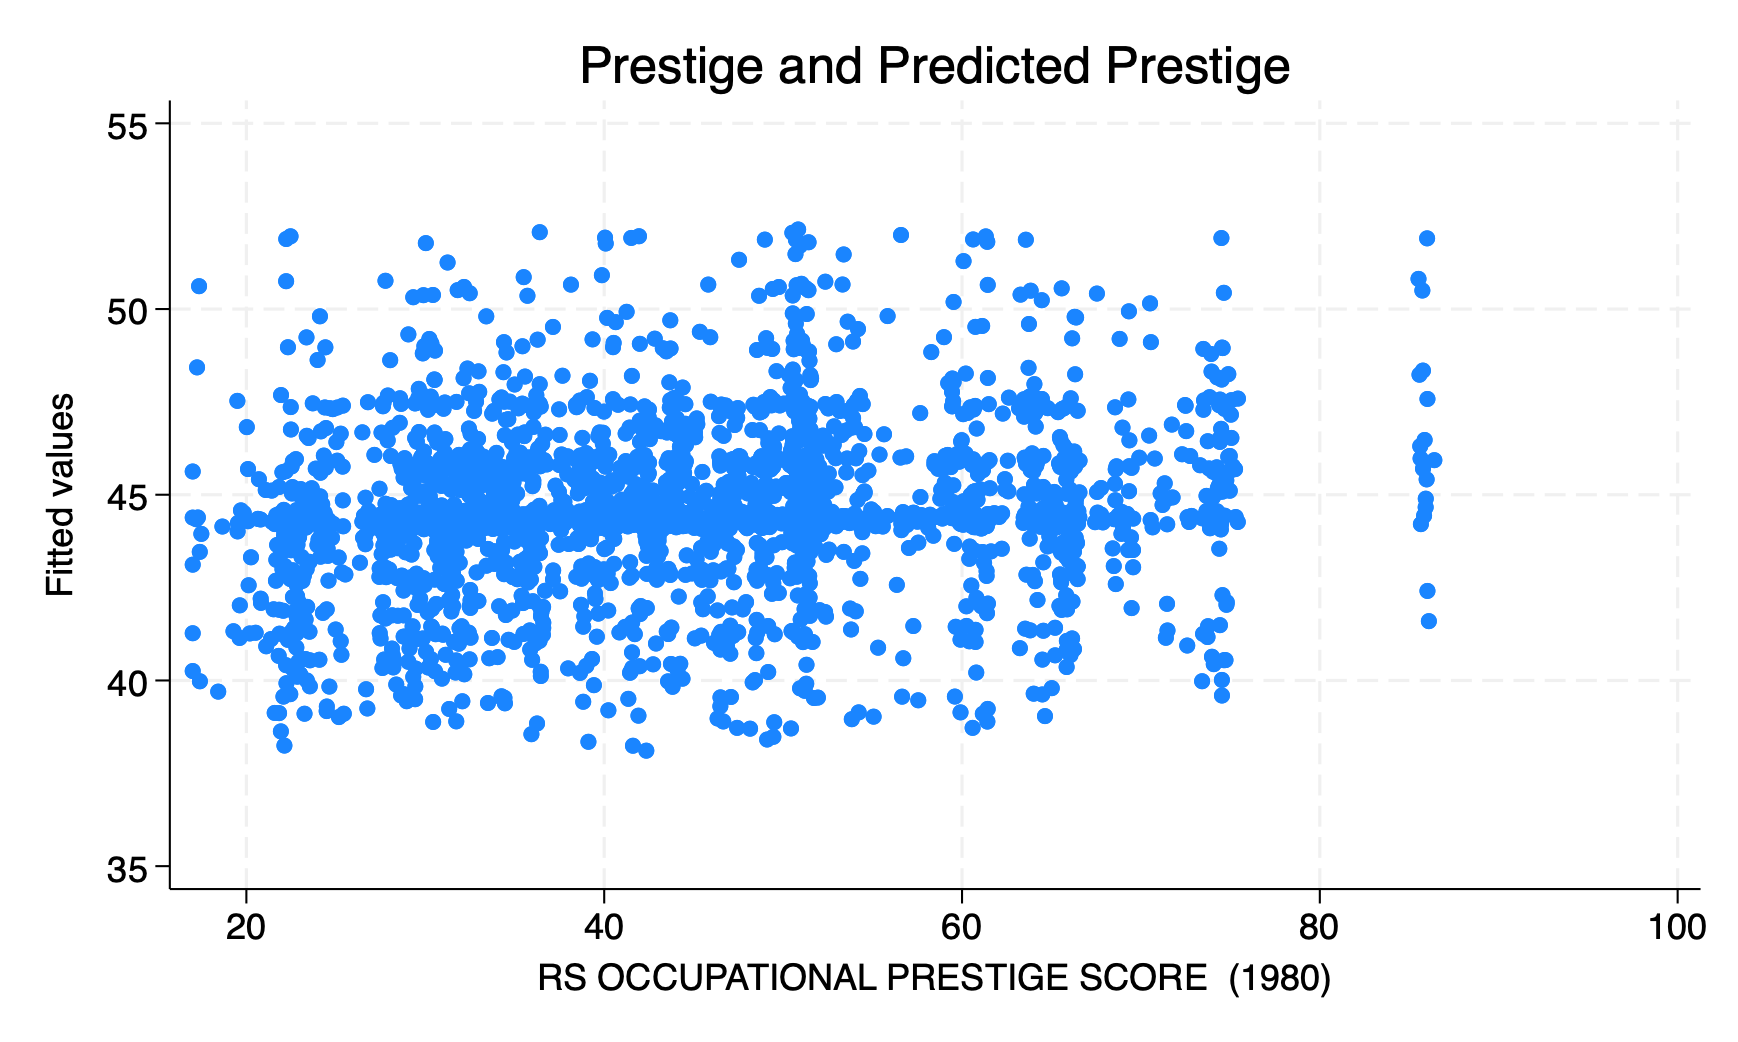
\includegraphics[keepaspectratio,alt={Scatterplot of Prestige and Predicted Prestige}]{Week12_4.png}}
\caption{Scatterplot of Prestige and Predicted Prestige}
\end{figure}

We can use a \textbf{twoway} using a \textbf{lfitci} line graph. The \emph{lfitci} will produce a simple bivariate linear regression between prestige and hours. It will also plot the confidence interval around the regression line.

\begin{Shaded}
\begin{Highlighting}[]
\KeywordTok{twoway}\NormalTok{ (lfitci prestg80 hrs1), }\DecValTok{scheme}\NormalTok{(s2mono) }\BaseNTok{title}\NormalTok{(}\StringTok{"Regress working hours onto prestige"}\NormalTok{) }\BaseNTok{caption}\NormalTok{(}\StringTok{"Source: General Social Survey of 2026"}\NormalTok{)}
\end{Highlighting}
\end{Shaded}

\begin{figure}
\centering
\pandocbounded{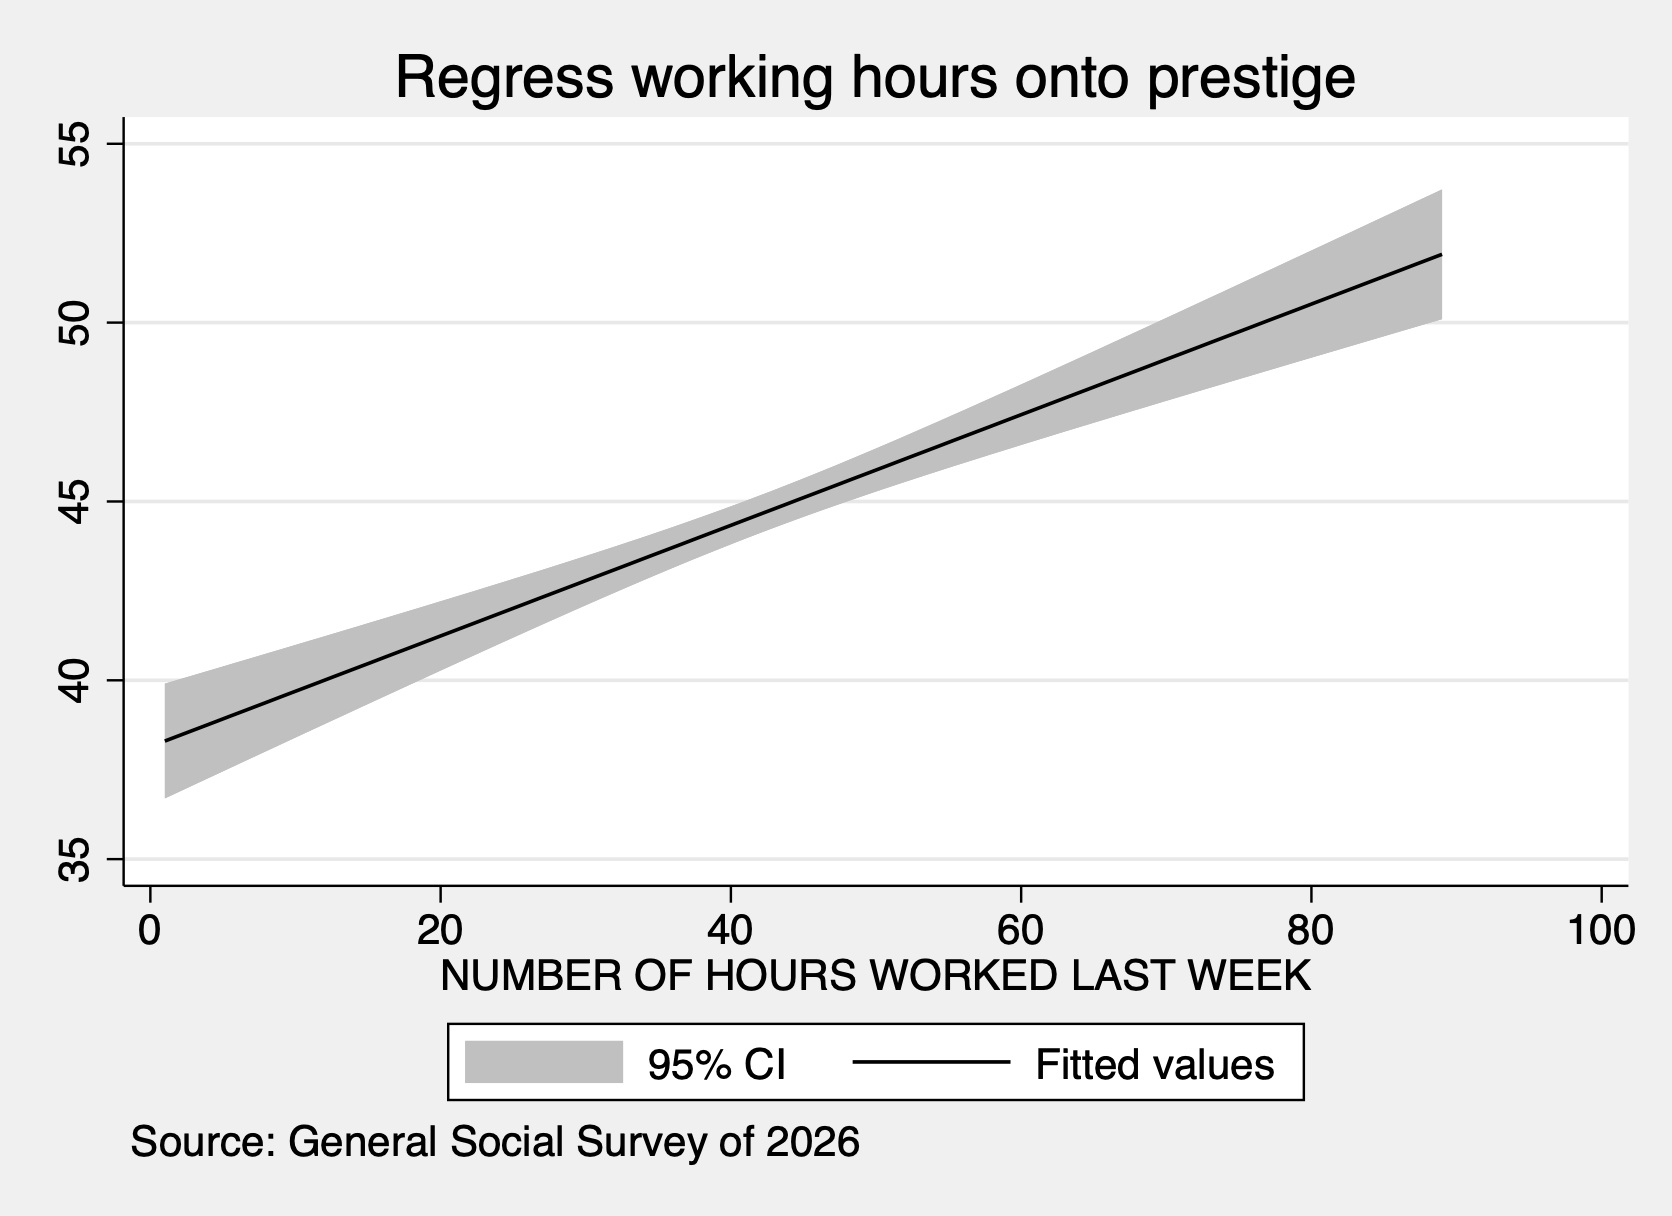
\includegraphics[keepaspectratio,alt={Regress working hours onto occupational prestige}]{Week12_1.png}}
\caption{Regress working hours onto occupational prestige}
\end{figure}

\section{Interpretations}\label{interpretations}

We have four way to interpret a simple linear regression depending on the transformation of the dependent or independent variable.

\begin{enumerate}
\def\labelenumi{\arabic{enumi}.}
\tightlist
\item
  Linear-linear model
\item
  Log-linear model.
\item
  Linear-log model.
\item
  Log-Log model
\end{enumerate}

First we need to create our natural log transformations of \(x\) and \(y\). We can use the \textbf{ln} function in Stata.

\begin{verbatim}
(4,510 missing values generated)

(2,739 real changes made)

(0 real changes made)

(4,510 missing values generated)

(4,270 real changes made)

(0 real changes made)

    Variable |        Obs        Mean    Std. dev.       Min        Max
-------------+---------------------------------------------------------
      lnhrs1 |      2,739    3.661178     .455948          0   4.488636
  lnprestg80 |      4,270    3.735998    .3278086   2.833213   4.454347
\end{verbatim}

Let's inspect the natural log transformation of prestige.

\begin{Shaded}
\begin{Highlighting}[]
\KeywordTok{histogram}\NormalTok{ lnprestg80, }\BaseNTok{title}\NormalTok{(}\StringTok{"Histogram of Natural Log of Prestige"}\NormalTok{)}
\end{Highlighting}
\end{Shaded}

\begin{figure}
\centering
\pandocbounded{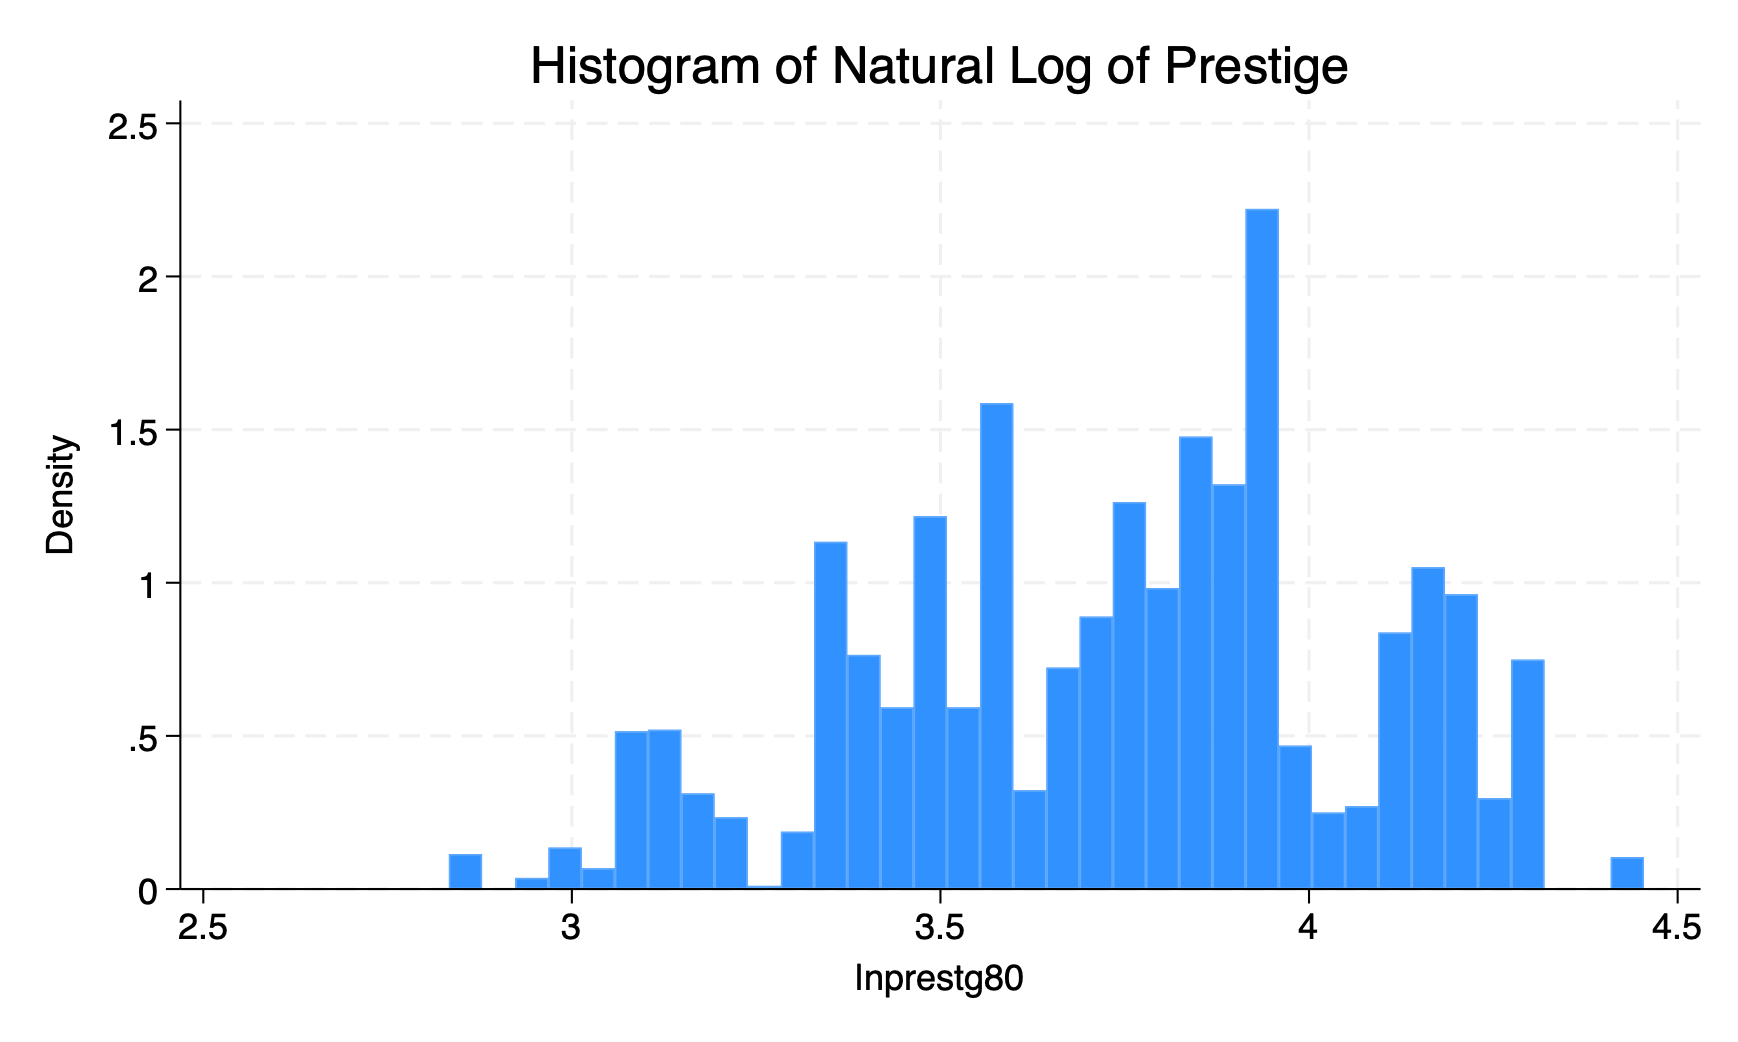
\includegraphics[keepaspectratio,alt={Histogram of Natural Log of Prestige}]{Week12_2.png}}
\caption{Histogram of Natural Log of Prestige}
\end{figure}

Next, let's inspect the natural log transformation of hours worked.

\begin{Shaded}
\begin{Highlighting}[]
\KeywordTok{histogram}\NormalTok{ lnhrs1, }\BaseNTok{title}\NormalTok{(}\StringTok{"Histogram of Natural Log of Hours"}\NormalTok{)}
\end{Highlighting}
\end{Shaded}

\begin{figure}
\centering
\pandocbounded{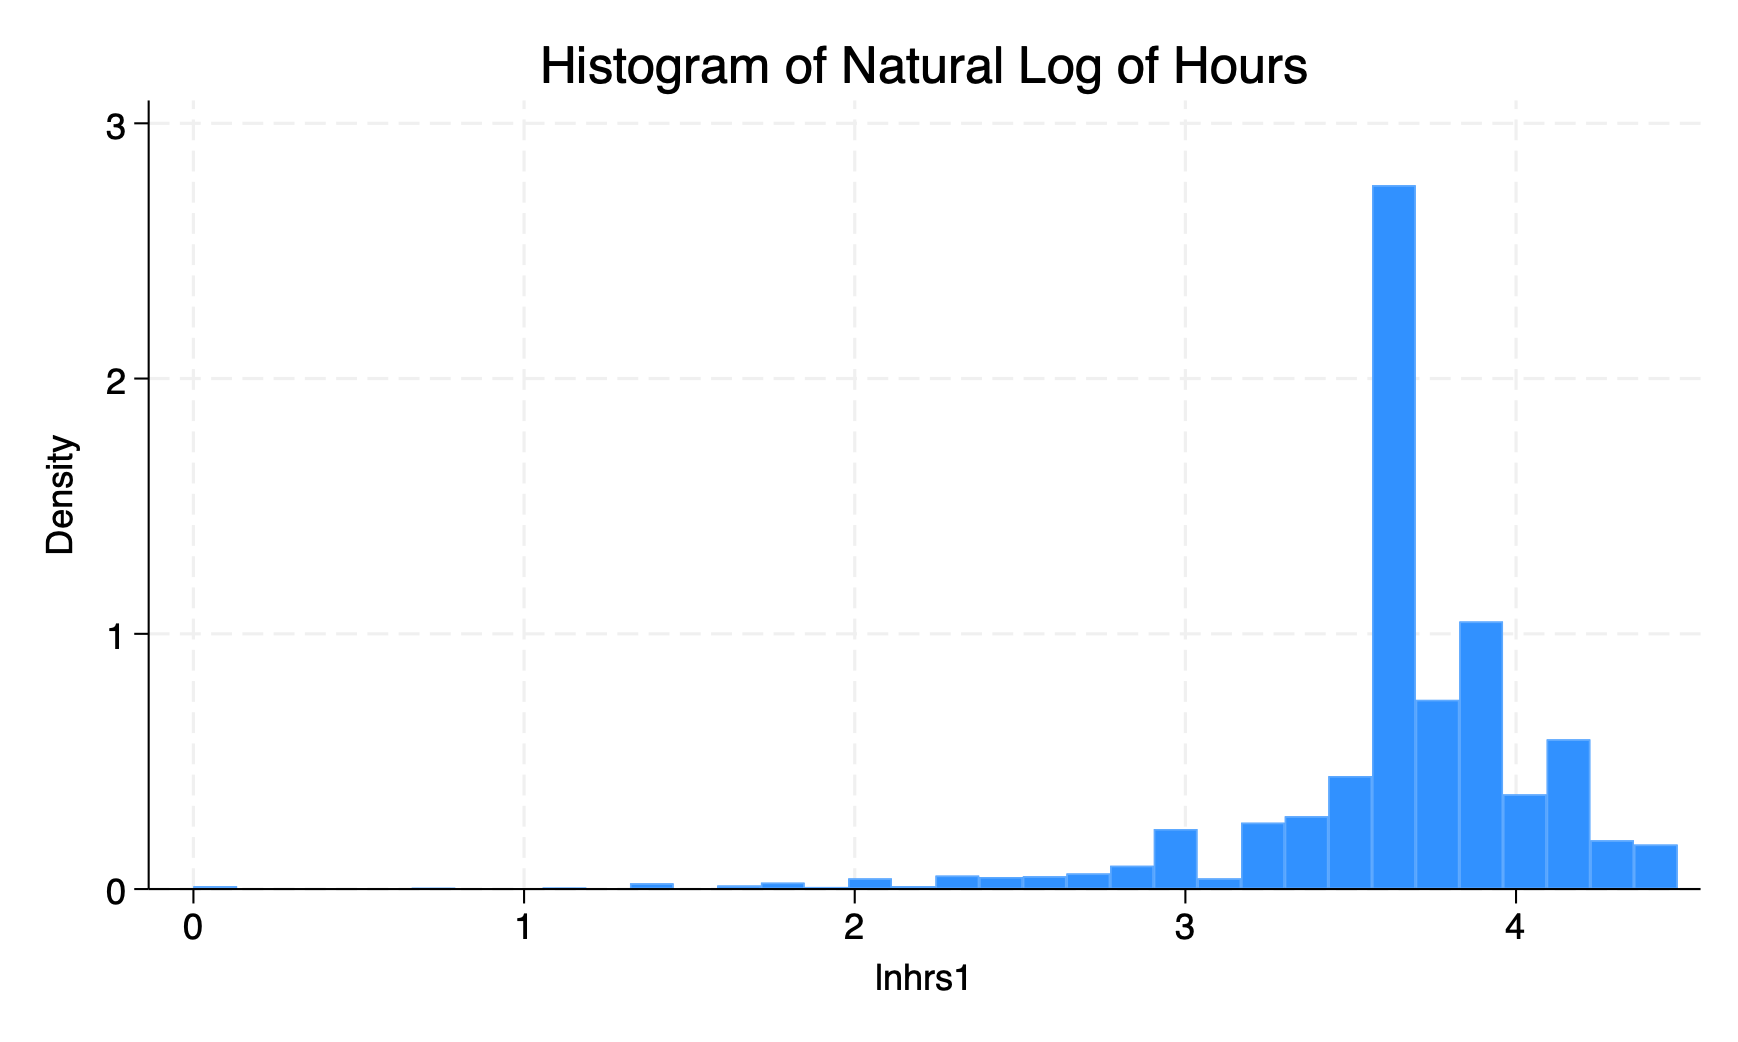
\includegraphics[keepaspectratio,alt={Histogram of the Natural Log of Hours}]{Week12_3.png}}
\caption{Histogram of the Natural Log of Hours}
\end{figure}

\subsection{Linear-Linear Model}\label{linear-linear-model}

\[ y_i = \beta_0 + \beta_1 x_i + \varepsilon_i \]

Let's rerun our linear-linear model and recall that \(\Delta y = \beta_1 \Delta x_1\), so we interpret \(\beta_1\) as a one-unit increase in \(x\) leads to a \(\beta_1\) increase in \(y\).

\begin{Shaded}
\begin{Highlighting}[]
\KeywordTok{regress}\NormalTok{ prestg80 hrs1}
\end{Highlighting}
\end{Shaded}

\begin{verbatim}
      Source |       SS           df       MS      Number of obs   =     2,715
-------------+----------------------------------   F(1, 2713)      =     67.32
       Model |   13125.035         1   13125.035   Prob > F        =    0.0000
    Residual |  528901.224     2,713  194.950691   R-squared       =    0.0242
-------------+----------------------------------   Adj R-squared   =    0.0239
       Total |  542026.259     2,714  199.714908   Root MSE        =    13.962

------------------------------------------------------------------------------
    prestg80 | Coefficient  Std. err.      t    P>|t|     [95% conf. interval]
-------------+----------------------------------------------------------------
        hrs1 |   .1546416   .0188468     8.21   0.000      .117686    .1915972
       _cons |   38.14733   .8362129    45.62   0.000     36.50765    39.78701
------------------------------------------------------------------------------
\end{verbatim}

We reject the null hypothesis that \(H_0: \beta_1 = 0\) at the 0.1\% level and we interpret this as a \(1\) hour increase is \textbf{associated} with a 0.155 increase in prestige.

Question: what does \(\beta_0\) represent?

\subsection{Linear-Log Model}\label{linear-log-model}

\[ y_i = \beta_0 + \beta_1 ln(x_i) + \varepsilon_i \]

Let's run a linear-log model where the dependent variable is not log transformed but the independent variable is log transformed.

We interpret \(\beta_1\) as a \(1\%\) increase in \(x\) is associated with a \(\frac{\beta_1}{100}\) increase in \(y\)

\begin{Shaded}
\begin{Highlighting}[]
\KeywordTok{regress}\NormalTok{ prestg80 lnhrs1}
\end{Highlighting}
\end{Shaded}

\begin{verbatim}
      Source |       SS           df       MS      Number of obs   =     2,715
-------------+----------------------------------   F(1, 2713)      =     48.89
       Model |  9594.06348         1  9594.06348   Prob > F        =    0.0000
    Residual |  532432.196     2,713  196.252192   R-squared       =    0.0177
-------------+----------------------------------   Adj R-squared   =    0.0173
       Total |  542026.259     2,714  199.714908   Root MSE        =    14.009

------------------------------------------------------------------------------
    prestg80 | Coefficient  Std. err.      t    P>|t|     [95% conf. interval]
-------------+----------------------------------------------------------------
      lnhrs1 |   4.115376   .5885935     6.99   0.000     2.961239    5.269513
       _cons |   29.58522   2.170863    13.63   0.000      25.3285    33.84193
------------------------------------------------------------------------------
\end{verbatim}

We reject the null hypothesis that \(H_0: \beta_1 = 0\) at the 0.1\% level and we interpret this as a \(1\%\) increase in hours is associated with a \(\frac{4.12}{100}=0.0412\) increase in prestige.

\subsection{Log-Linear Model}\label{log-linear-model}

\[ ln(y_i) = \beta_0 + \beta_1 x_i + \varepsilon_i \]

Let's run a log-linear model, where the dependent variable is log transformed but the independent variable is not log transformed.

We interpret this as a interpret \(\beta_1\) as a 1-unit increase in \(x\) is associated with a \((e^{\beta_{1}}-1)*100 \%\) increase in \(y\).

\begin{Shaded}
\begin{Highlighting}[]
\KeywordTok{regress}\NormalTok{ lnprestg80 hrs1}
\end{Highlighting}
\end{Shaded}

\begin{verbatim}
      Source |       SS           df       MS      Number of obs   =     2,715
-------------+----------------------------------   F(1, 2713)      =     75.24
       Model |  7.87166582         1  7.87166582   Prob > F        =    0.0000
    Residual |  283.847275     2,713  .104624871   R-squared       =    0.0270
-------------+----------------------------------   Adj R-squared   =    0.0266
       Total |  291.718941     2,714  .107486714   Root MSE        =    .32346

------------------------------------------------------------------------------
  lnprestg80 | Coefficient  Std. err.      t    P>|t|     [95% conf. interval]
-------------+----------------------------------------------------------------
        hrs1 |   .0037871   .0004366     8.67   0.000      .002931    .0046432
       _cons |   3.587671   .0193719   185.20   0.000     3.549686    3.625656
------------------------------------------------------------------------------
\end{verbatim}

We reject the null hypothesis that \(H_0: \beta_1 = 0\) at the 0.1\% level and we interpret that a 1-unit increase in hours is \textbf{associated} with a \((e^{.0037871}-1)*100 \% = .38\%\) increase in occupational prestige.

\subsection{Log-Log Model}\label{log-log-model}

With a log-log model, we interpret A 1\% increase in years of education is associated with a 𝛽\_1\% change in wages

\[ ln(y_i) = \beta_0 + \beta_1 ln(x_i) + \varepsilon_i \]

We interpret \(\beta\) as a 1\% increase in \(x\) is associated with a \(\beta_1\%\) change in \(y\).

\begin{Shaded}
\begin{Highlighting}[]
\KeywordTok{regress}\NormalTok{ lnprestg80 lnhrs1}
\end{Highlighting}
\end{Shaded}

\begin{verbatim}
      Source |       SS           df       MS      Number of obs   =     2,715
-------------+----------------------------------   F(1, 2713)      =     57.58
       Model |  6.06313896         1  6.06313896   Prob > F        =    0.0000
    Residual |  285.655802     2,713  .105291486   R-squared       =    0.0208
-------------+----------------------------------   Adj R-squared   =    0.0204
       Total |  291.718941     2,714  .107486714   Root MSE        =    .32449

------------------------------------------------------------------------------
  lnprestg80 | Coefficient  Std. err.      t    P>|t|     [95% conf. interval]
-------------+----------------------------------------------------------------
      lnhrs1 |   .1034563   .0136334     7.59   0.000     .0767234    .1301892
       _cons |   3.368208   .0502831    66.98   0.000     3.269611    3.466805
------------------------------------------------------------------------------
\end{verbatim}

We reject the null hypothesis that \(H_0: \beta_1 = 0\) at the 0.1\% level and we interpret this as a \(1\%\) increase in hours is associated with a \(0.1\%\) increase in occupational prestige.

\chapter{Exercises}\label{exercises}

\section{General Social Survey}\label{general-social-survey}

Let's implement the following model based on the General Social Survey.

\[ prestg80_i = \beta_0 + \beta_1 educ_i + \varepsilon_i \]

Steps:

\begin{enumerate}
\def\labelenumi{\arabic{enumi}.}
\tightlist
\item
  Set up a hypothesis about education and occupational prestige
\item
  Summarize prestige and education.
\item
  Regress prestige onto education.
\item
  What is \(\beta_1\)?
\item
  Interpret your finding.
\item
  What do you conclude?
\end{enumerate}

\section{Current Population Survey}\label{current-population-survey}

Let's look at the following model based on the Current Population Survey.

\[ earnings_i = \beta_0 + \beta_1 educ_i + \varepsilon_i \]

Steps:

\begin{enumerate}
\def\labelenumi{\arabic{enumi}.}
\tightlist
\item
  Import the 2024 CPS data from NBER Merged Outgoing Rotation Group \url{https://data.nber.org/morg/annual/}
\item
  Summarize weekly earnings (earnwke) and imputed education (ihigrdc)
\item
  Regress earnings onto education
\item
  What is \(\beta_1\)?
\item
  Interpret your findings.
\item
  What do you conclude?
\item
  Take the natural log of earnings.
\item
  Regress \(ln(earnwke)\) onto education.
\item
  Interpret your findings.
\end{enumerate}

Acock, A.C. (2023). A gentle introduction to Stata. 6th ed.~Stata Press.

Anderson, D. R., Sweeney, D. J., Williams, T. A., Camm, J. D., \& Cochran, J. J. (2016). Statistics for business and economics (13th ed.). Cengage Learning.

Mitchell, M. N. (2020). Data management using Stata: A practical handbook. Stata Press.

\bibliography{book.bib,packages.bib}

\end{document}
